\documentclass[10pt,landscape,a4paper]{article}
\usepackage[english]{babel}
\usepackage[utf8]{inputenc}
\usepackage[plain]{algorithm}
\usepackage[noend]{algpseudocode}
\usepackage{tikz}
\usepackage{pgfplots}
\usepackage{palatino}
\usepackage{multicol}
\usepackage{blkarray}

\usepackage{calc}
\usepackage{ifthen}
\usepackage[landscape]{geometry}
\usepackage{graphicx}
\usepackage{amsmath, amssymb, amsthm}
\DeclareMathOperator*{\argmin}{argmin}
\DeclareMathOperator*{\argmax}{argmax}

\usepackage{physics}
\usepackage{latexsym, marvosym}
\usepackage{pifont}
\usepackage{lscape}
\usepackage{dsfont}
\usepackage{graphicx}
\usepackage{array}
\usepackage{booktabs}
\usepackage[bottom]{footmisc}
\usepackage{tikz}
\usetikzlibrary{shapes}
\usepackage{pdfpages}
\usepackage{wrapfig}
\usepackage{enumitem}
\setlist[description]{leftmargin=0pt}
\usepackage{xfrac}
\usepackage[pdftex,
            pdfauthor={Jose},
            pdftitle={Foundations of Modern Finance I},
            pdfsubject={Cheat sheet for MITx: 15.415.1x Foundations of Modern Finance I.},
            pdfkeywords={finance} {cheatsheet} {pdf} {cheat} {sheet} {formulas} {equations}
            ]{hyperref}
\usepackage[
            open,
            openlevel=2
            ]{bookmark}
\usepackage{relsize}
\usepackage{rotating}

% for monospace font https://tex.stackexchange.com/questions/50810/good-monospace-font-for-code-in-latex
\usepackage{inconsolata}


 \newcommand\independent{\protect\mathpalette{\protect\independenT}{\perp}}
    \def\independenT#1#2{\mathrel{\setbox0\hbox{$#1#2$}%
    \copy0\kern-\wd0\mkern4mu\box0}} 
            
\newcommand{\noin}{\noindent}    
\newcommand{\logit}{\textrm{logit}} 
%\newcommand{\var}{\textrm{Var}}
\newcommand{\cov}{\textrm{Cov}} 
\newcommand{\corr}{\textrm{Corr}} 
\newcommand{\N}{\mathcal{N}}
\newcommand{\Bern}{\textrm{Bern}}
\newcommand{\Bin}{\textrm{Bin}}
\newcommand{\Beta}{\textrm{Beta}}
\newcommand{\Gam}{\textrm{Gamma}}
\newcommand{\Expo}{\textrm{Expo}}
\newcommand{\Pois}{\textrm{Pois}}
\newcommand{\Unif}{\textrm{Unif}}
\newcommand{\Geom}{\textrm{Geom}}
\newcommand{\NBin}{\textrm{NBin}}
\newcommand{\Hypergeometric}{\textrm{HGeom}}
\newcommand{\HGeom}{\textrm{HGeom}}
\newcommand{\Mult}{\textrm{Mult}}

\geometry{top=.4in,left=.2in,right=.2in,bottom=.4in}

\pagestyle{empty}
\makeatletter
\renewcommand{\section}{\@startsection{section}{1}{0mm}%
                                {-1ex plus -.5ex minus -.2ex}%
                                {0.5ex plus .2ex}%x
                                {\normalfont\large\bfseries}}
\renewcommand{\subsection}{\@startsection{subsection}{2}{0mm}%
                                {-1explus -.5ex minus -.2ex}%
                                {0.5ex plus .2ex}%
                                {\normalfont\normalsize\bfseries}}
\renewcommand{\subsubsection}{\@startsection{subsubsection}{3}{0mm}%
                                {-1ex plus -.5ex minus -.2ex}%
                                {1ex plus .2ex}%
                                {\normalfont\small\bfseries}}
\makeatother

\setcounter{secnumdepth}{0}

\setlength{\parindent}{0pt}
\setlength{\parskip}{0pt plus 0ex}

% -----------------------------------------------------------------------

\usepackage{titlesec}

\titleformat{\section}
{\color{blue}\normalfont\normalsize\bfseries}
{\color{blue}\thesection}{0em}{}
\titleformat{\subsection}
{\color{violet}\normalfont\normalsize\bfseries}
{\color{violet}\thesection}{1em}{}
% Comment out the above 5 lines for black and white

\begin{document}

\raggedright
\footnotesize
\begin{multicols*}{3}

% multicol parameters
% These lengths are set only within the two main columns
%\setlength{\columnseprule}{0.25pt}
\setlength{\premulticols}{1pt}
\setlength{\postmulticols}{1pt}
\setlength{\multicolsep}{1pt}
\setlength{\columnsep}{1pt}

%%%%%%%%%%%%%%%%%%%%%%%%%%%%%%%%%%%%
%%% TITLE
%%%%%%%%%%%%%%%%%%%%%%%%%%%%%%%%%%%%

\begin{center}
    {\color{blue} \Large{\textbf{Foundations of Modern Finance I}}} \\
   % {\Large{\textbf{Foundations of Modern Finance I}}} \\
    % comment out line with \color{blue} and uncomment above line for b&w
\end{center}

%%%%%%%%%%%%%%%%%%%%%%%%%%%%%%%%%%%%
%%% ATTRIBUTIONS
%%%%%%%%%%%%%%%%%%%%%%%%%%%%%%%%%%%%

\scriptsize

Cheat sheet for MITx: 15.415.1x Foundations of Modern Finance I.


% Cheatsheet format from
% http://www.stdout.org/$\sim$winston/latex/

%%%%%%%%%%%%%%%%%%%%%%%%%%%%%%%%%%%%
%%% BEGIN CHEATSHEET
%%%%%%%%%%%%%%%%%%%%%%%%%%%%%%%%%%%%


\section{Week 2: Market Prices and Present Value}\smallskip \hrule height 1pt \smallskip


\subsection{State-space model for time and risk}

\begin{description}[itemsep=0pt]
	\item[State-space model] ~
	\begin{itemize}
		\item Assets can be traded at time $t = 0$ with payoffs at time $t = 1$.
		\item The price of an asset is $P$ at $t= 0$ with payoff $X=(X_1, \dots , X_N)$ at $t=1$.
		\item $X$ is a random variable.
		\item A random payoff is given by the value of	its payoff in each state and the corresponding probability:
		$[(X_1, \dots, X_N); (p_1, \dots , p_N)] $
		\item{\bf expected} value : $\sum_{i=1}^{N} p_i X_i$ 
	\end{itemize}
	\item[State Prices]~
	\begin{itemize}
		\item Consider primitive state-contingent claims (Arrow-Debreu securities) that pay \$1 in a	single state and nothing otherwise.
		\item Denote the price of the A-D claim on state $j$ by $\phi_j$ , the state price for state $j$.
		\item No arbitrage requires that all state prices must be positive: $\phi_j > 0$ for all $j$.
		\item The market is called complete if one can effectively trade A-D securities on each state.
	\end{itemize}	
\end{description}


\subsection{Arbitrage pricing}

\begin{description}[itemsep=0pt]
	\item[Arbitrage pricing] ~
	\begin{itemize}
		\item With the prices of A-D securities, we can price other assets/securities.
		\item Law of One Price: Two assets with the same payoff must have the same	market price.
		\item Suppose the firm is considering a project yielding time-1 cash flow: $X=(X_1, X_2, \dots, X_N)$
		\item Using prices of A-D securities, we can attach {\bf market value} to this cash flow as: $P = \phi_1 X_1 + \dots +\phi_N X_N = PV $
		\item Example for three assets: riskless bonds pays \$100 in each state currently traded at $B1_0$, stock 1 pays off $[S1_1, S1_2, S1_3]$ and currently traded at $S1_0$, 
		 stock 2 pays off $[S2_1, S2_2, S2_3]$ and currently traded at $S2_0$:
		$$
		\begin{pmatrix}
			100 & 100 & 100   \\
			S1_1 & S1_2 & S1_3 \\
			S2_1 & S2_2 & S3_3 \\							
		\end{pmatrix} \cdot 
		\begin{pmatrix}
			\phi_1 \\
			\phi_2 \\
			\phi_3 \\								
		\end{pmatrix}	
		=
		\begin{pmatrix}
			B1_0\\
			S1_0 \\
			S2_0 \\								
		\end{pmatrix}
		$$ 
		solve system to find state prices $\phi_1$, $\phi_2$, $\phi_3$.	 
	\end{itemize}	
\end{description}

\subsection{Present value and future value}

\begin{description}[itemsep=0pt]
	\item[Present value and discount rate] ~
	\begin{itemize}
		\item $PV = \frac{E[CF]}{1 + \bar{r}} $
	\end{itemize}	
	\item[Future Value] ~
	\begin{itemize}
		\item $FV$ in $T$ years: $FV=(1 + r)^T$
	\end{itemize}
\end{description}

\subsection{Nominal vs. real cash flows and returns}

\begin{description}[itemsep=0pt]
	\item[Nominal vs real CFs] ~
	\begin{itemize}
		\item Nominal cash flows $\implies$ expressed in actual-dollar cash flows.
		\item Real cash flows $\implies$ expressed in constant purchasing power.
		\item At an annual inflation rate of $i$, we have:  $(Real CF)_t = \frac{(Nominal CF)_t}{(1+i)^t}$
	\end{itemize}	
	\item[Nominal vs real rates] ~
	\begin{itemize}
		\item Nominal rates of return $\implies$ prevailing market rates.
		\item Real rates of return $\implies$ inflation adjusted rates
		\item Real rate of return:  $r_{real} = \frac{1+r_{nominal}}{1+i} -1 \approx r_{nominal}-i$
	\end{itemize}
\end{description}





\section{Week 3: Discounting and Compounding}\smallskip \hrule height 1pt \smallskip


\subsection{Special Cash Flows}

\begin{description}[itemsep=0pt]
	\item[Special Cash Flows] ~
	\begin{itemize}
		\item {\bf Annuity:}
		$ PV = A \cdot \frac{1}{r} \Big[\ 1-\frac{1}{(1+r)^T} \Big] $
		$	FV = PV \cdot (1+r)^T $
		\item {\bf Annuity with constant growth:} 
		$$ PV =
		\begin{cases}
		$$A \cdot \frac{1}{r-g} \Big[ 1- \left( \frac{1+g}{1+r} \right) ^T  \Big]$$ \quad\text{if }  $$ r \neq g $$ \\
		$$A \cdot \frac{T}{1+r}$$ \quad\text{if }  $$ r=g $$
		\end{cases}$$
		\item {\bf Perpetuity:}
		$PV = \frac{A}{r}$
		\item {\bf Perpetuity with constant growth:} 
		$ PV = \frac{A}{r-g}  \text{,}\quad r>g$
	\end{itemize}
\end{description}

\subsection{Compounding}
\begin{description}[itemsep=0pt]
	\item[APR / EAR]  ~
	\begin{itemize}
		\item {\bf EAR:Effective Annual Rate} $ r_{EAR} = \left( 1+\frac{r_{APR}}{k} \right)^k-1 $
		\item {\bf APR:Annual Percentage Rate} $ r_{APR} = k \left[\left( 1+r_{EAR} \right)^ {\frac{1}{k}}-1 \right] $
	\end{itemize}
\end{description}



\section{Week 4: Fixed Income Securities}\smallskip \hrule height 1pt \smallskip


\subsection{Relative Bond Valuation}
\begin{description}[itemsep=0pt]
	\item[Arbitrage]  ~
	\begin{itemize}
		\item {\bf Arbitrage: } The key is to construct the payoffs so that we get \$100 in year 0 
		and we get \$0 payoffs in all of the subsequent years, i.e. the cashflows of the bonds should offset each other at all times except year 0 when we realize the arbitrage of \$100. For example, suppose there are three bonds with prices $P_1$, $P_2$ and $P_2$ with maturities 1, 2 and 3 years and coupons $C_1$, $C_2$, $C_3$, respectively, and all with face value $F$. There is a fourth bond with price $P_4$ and coupon $C_4$ with maturity 3 years (adjust cashflows if maturity is not 3 years) undervalued or overvalued. In order to find the arbitrage strategy we need to solve the following system of equations:
		$$
		\begin{pmatrix}
			-P_1 & -P_2 & -P_3  & -P_4\\
			C_1+F & C_2 & C_3 & C_4 \\
			0 & C_2+F & C_3 & C_4 \\
			0 & 0 & C_3+F & C_4+F \\								
		\end{pmatrix} \cdot 
		\begin{pmatrix}
			X_1\\
			X_2 \\
			X_3 \\
			X_4 \\									
		\end{pmatrix}	
		=
		\begin{pmatrix}
		100\\
		0 \\
		0 \\
     	0 \\									
		\end{pmatrix}
		$$ In matrix notation:  
		$A \cdot X = B  \implies X = A^{-1}\cdot B$ \\
	{
\includegraphics[width=0.15in]{images/excel_logo.png}} \texttt{ X=MMULT(MINVERSE(A),B)}
	\end{itemize}
\end{description}


\subsection{Interest Risk, Bond Duration and Bond Convexity}
\begin{description}[itemsep=0pt]
	\item[Bond Duration]  ~
	\begin{itemize}
		\item {\bf Modified Duration (MD) for discount bond $ B_t=\frac{1}{(1+y)^t} $ } $$ MD(B_t) = -\frac{1}{B_t}\frac{dB_t}{dy} = \frac{t}{1+y}$$
		\item {\bf Macaulay Duration} is the weighted average term to maturity  $$ D = \sum_{t=1}^{T} \left(   \frac{PV(CF_T)}{B}  t \right)  =   \frac{1}{B}\sum_{t=1}^{T} \left(  \frac{CF_t}{(1+y)^t} t \right)  $$
		\item {\bf Modified Duration} measures bond's interest rate risk by its relative price change with respect
		to a unit change in yield (with a negative sign):  $$ MD =  -\frac{1}{B}\frac{dB}{dy}  = \frac{D}{1+y}  $$
		\item {\bf Convexity (CX)} measure the curvature of the bond price as function of the yield:  $$ CX =  \frac{1}{2}\frac{1}{B}\frac{d^2B}{dy^2}  $$
		\item {\bf Taylor series approximation of bond price changes}  $$ \Delta B \approx  B \left(  -MD  \cdot \Delta y + CX \cdot ( \Delta y)^2 \right)    $$
	\end{itemize}
\end{description}


\section{Week 5: Stocks}\smallskip \hrule height 1pt \smallskip


\subsection{Growth Opportunities and Stock Valuation}

\begin{description}[itemsep=0pt]
	\item[P/E and PVGO: price/earning and present value of growth opportunities]  ~
	\begin{itemize}
		\item {\bf P/E and PVGO:} $ P_0 = \frac{EPS_1}{r} + PVGO $
		\item {\bf if $PVGO=0$:} $ P/E = \frac{1}{r}  $
		\item {\bf if $PVGO>0$:} $ P/E = \frac{1}{r} + \frac{PVGO}{EPS_2} > \frac{1}{r} $
	\end{itemize}
\end{description}



\subsection{Investment and Growth}

\begin{description}[itemsep=0pt]
	\item[plow-back ratio $b_t$]  ~
	\begin{itemize}
		\item {\bf Investments:} $ I_t = EPS_t \cdot b_t $
		\item {\bf Next year earnings} $ EPS_{t+1} = EPS_t +ROI_t \cdot I_t $
		\item {\bf Next year book value:} $ BVPS_{t+1} = BVPS_t + I_{t+1} $
		\item {\bf Dividedns:} $ D_t = EPS_t (1-b_t) $
		
			
	\end{itemize}
\end{description}



\section{Week 6: Risk}\smallskip \hrule height 1pt \smallskip

\begin{description}[itemsep=0pt]
	\item[Portfolio mean and variance, two assets]  ~
	\begin{itemize}
		\item {\bf Expected portfolio return:} $ \bar{r}_p = w_1 \bar{r}_1 +  w_2 \bar{r}_2 $
		\item {\bf Unexpected portfolio return:} $ \tilde{r}_p - \bar{r}_p= w_1 (\tilde{r}_1 - \bar{r}_1) +  w_2 (\tilde{r}_2 - \bar{r}_2) $
		\item {\bf The variance of the portfolio return:} $ \sigma_p^2 = w_1^2 \sigma_1^2 + w_2^2 \sigma_2^2 + 2 w_1 w_2 \sigma_{12}  $ \\
													      $ \sigma_p^2 = w_1^2 \sigma_1^2 + w_2^2 \sigma_2^2 + 2 w_1 w_2 \rho_{12} \sigma_1 \sigma_2  $		
		\item {\bf Correlation and covariance:} $  \rho_{12} = \frac{\sigma_{12}}{\sigma_1 \sigma_2}$	
	\end{itemize}
\end{description}






\section{Week 7: Arbitrage Pricing Theory}\smallskip \hrule height 1pt \smallskip


\subsection{Factor Models}

\begin{description}[itemsep=0pt]
	\item[A single-factor model]  ~
	\begin{itemize}
		\item {\bf Asset returns:} $ \tilde{r}_i = \underbrace{\bar{r}_i}_{\substack{\text{expected} \\ \text{return}}} +  \underbrace{b_i \tilde{f} + \tilde{\epsilon}_i}_{\text{risk}} $
		\item {\bf Return variance:} $ \sigma_i^2 = \underbrace{b_i^2 \sigma_f^2}_{\substack{\text{systematic} \\ \text{risk}}} +  \underbrace{Var(\tilde{\epsilon}_i)}_{\substack{\text{idiosyncratic} \\ \text{risk}}} $
		\item {\bf Return covariance:} $ Cov( \tilde{r}_i,  \tilde{r}_j) = Cov(b_i \tilde{f} + \tilde{\epsilon}_i, b_j \tilde{f} + \tilde{\epsilon}_j) = b_i b_j \sigma_f^2 $ because of the assumptions:
		$Cov(\tilde{f}, \tilde{\epsilon}_i ) = 0$
		$Cov( \tilde{\epsilon}_i , \tilde{\epsilon}_j ) = 0$
			
	\end{itemize}
\end{description}

\begin{description}[itemsep=0pt]
	\item[Two-factor model]  ~
	\begin{itemize}
		\item {\bf Asset returns:} $ E[\tilde{r}_i] - r_f =  b_{i1} \lambda_1 + b_{i2} \lambda_2 $
		\item {\bf Return variance:} $ \sigma_i = \sqrt{ b_{i,1}^2 Var[f_1] +  b_{i,2}^2 Var[f_2] + Var[\tilde{u}_i}]$
		\item {\bf Return covariance:} $ Cov_{1,2} =  b_{1,1} b_{1,2} Var[f_1]  +  b_{1,2} b_{2,2} Var[f_2]$
		\item {\bf Return correlation:} $ Corr_{1,2} = \frac{Cov_{1,2}}{\sigma_1 \sigma_2}$
		
	\end{itemize}
\end{description}


\begin{description}[itemsep=0pt]
	\item[Multifactor models]  ~
	\begin{itemize}
		\item {\bf Asset returns:} $ \tilde{r}_i = \underbrace{\bar{r}_i}_{\text{expected return}} +  \underbrace{b_{i,1} \tilde{f}_1 + b_{i,2} \tilde{f}_1 + \dots + b_{i,K} \tilde{f}_K }_{\text{systematic component}}  +\tilde{\epsilon}_i $

		\item {\bf Assumptions:} 
		$Cov( \tilde{\epsilon}_i , \tilde{\epsilon}_j ) = 0 \text{, } \forall{i \neq j} $ \\
		$E[\tilde{f}_k]=0 \text{, } k=1,2, \dots , K $
		
	\end{itemize}
\end{description}

\begin{description}[itemsep=0pt]
	\item[Portfolio return]  ~
	\begin{itemize}
		\item {\bf Portfolio return:} $$ \tilde{r}_p = \bar{r}_p +  b_{p,1} \tilde{f}_1 + b_{p,2} \tilde{f}_1 + \dots + b_{p,K} \tilde{f}_K  +\tilde{\epsilon}_p $$
		where, 
		$$ \bar{r}_p = \sum_{i=1}^{N}{w_i \bar{r}_i}  \quad   b_{p,k}=\sum_{i=1}^{N}{w_i b_{i,k}} \quad  \tilde{\epsilon}_p = \sum_{i=1}^{N}{w_i \tilde{\epsilon}_i}$$
		\item {\bf Non-systematic variance:} $$ Var( \tilde{\epsilon}_p) = Var \left( \sum_{i=1}^{N}{w_i \tilde{\epsilon}_i}  \right) = \sum_{i=1}^{N}{w_i ^2 Var (\tilde{\epsilon}_i)} $$
		
	\end{itemize}
\end{description}


\begin{description}[itemsep=0pt]
	\item[Expected Returns on Diversified Portfolios]  ~
	\begin{itemize}
		\item {\bf APT pricing relation:} $$ \underbrace{\tilde{r}_p - \bar{r}_f}_{\text{Risk premium}} =  \underbrace{\lambda}_{\text{Price of risk}} \cdot \underbrace{b_p}_{\text{Quantity of risk}} $$ $\lambda$ tells us how much compensation one earns in the market for a unit of
		factor risk exposure. $\lambda$ is called the market price of risk of the factor, or the factor risk premium.
	   \item {\bf APT relation for multi-factor models:} $$ \tilde{r}_p - \bar{r}_f = \lambda_1 b_{p,1} + \lambda_2 b_{p,2} + \dots + \lambda_K b_{p,K} $$
		
	\end{itemize}
\end{description}




\section{Week 8: Market Efficiency}\smallskip \hrule height 1pt \smallskip

\begin{description}[itemsep=0pt]
	\item[Three forms of market efficiency hypothesis MEH]  ~
	\begin{itemize}
\item {\bf Weak-form efficiency}: security prices reflect all information contained in past prices $\implies$ Technical analysis does not provide excess returns.
\item {\bf Semi-strong-form efficiency} : security prices reflect all publicly available information $\implies$ Fundamental analysis does not provide excess returns.
\item {\bf Strong-form efficiency }: security prices reflect all information, whether publicly available or not $\implies$  Inside information does not provide excess returns.		
	\end{itemize}
\end{description}

$ \text{Strong-form EMH} \implies \text{Semistrong-form EMH} \implies \text{Weak-form EMH}  $
	\begin{center}
	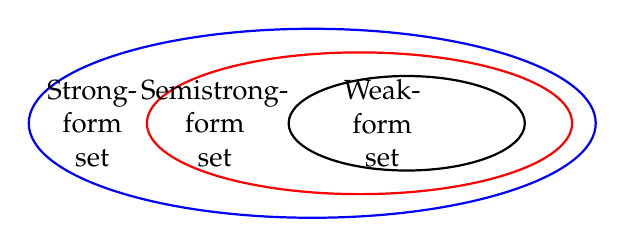
\begin{tikzpicture}[scale=0.6]
		\draw[blue, thick] (4.5,3) ellipse (6 and 2);
		\node[left, align=center] at (1,3) {Strong-\\form\\set };
		\draw[red, thick] (5.5,3) ellipse (4.5 and 1.5);
		\node[left, align=center] at (4.2,3) {Semistrong-\\form\\set };
		\draw[black, thick] (6.5,3) ellipse (2.5 and 1);
		\node[left, align=center] at (7,3) {Weak-\\form\\set };		
	\end{tikzpicture}
\end{center}




\section{Week 9: Introduction to Corporate Finance}\smallskip \hrule height 1pt \smallskip

\begin{description}[itemsep=0pt]
	\item[What is corporate finance?]  ~
	\begin{itemize}
		\item {\bf Capital budgeting}: What projects (real investments) to invest in? Expansions, new products, new businesses, acquisitions, ...
		\item {\bf  Financing}: How to finance a project? Selling financial assets/securities/claims (bank loans, public debt, stocks, convertibles, ...)
		\item {\bf Payout} : What to pay back to shareholders? Paying dividends, buyback shares, ...
		\item {\bf Risk management}: What risk to take/to avoid and how?	
	\end{itemize}
	\item[Task of financial manager]  ~
		\item Asset side (LHS): Real investments.
		\item Liability side (RHS): Financing, payout and risk management.

\end{description}

\section{Week 10: Capital Budgeting 1}\smallskip \hrule height 1pt \smallskip


\subsection{NPV Rule}

\begin{description}[itemsep=0pt]
	\item[Investment Criteria for NPV and cash flow calculations]  ~
	\begin{itemize}
		\item {\bf For a single project:} Take it if and only if its NPV is positive.
		\item {\bf For many independent projects:}  Take all those with positive NPV.
		\item {\bf For mutually exclusive projects:}  Take the one with positive and highest NPV.
		\item {\bf NPV:} $$ NPV = CF_0 + \frac{CF_1}{1+r_1}+\frac{CF_2}{(1+r_2)^2} + \cdots + \frac{CF_T}{(1+r_T)^T} $$
		\item {\bf Operating Profit:}
			 \begin{align*}
			 	 OperatingProfits &=  OperatingRevenues \\
			 	                  &- OperatingExpensesWithoutDepreciation
		 	 \end{align*}
		\item {\bf Cash Flow:} 
			\begin{align*}
				 CF &= (1-\tau) (OperatingProfits) - CapEx + \tau \cdot Depreciation \\
				  &-\Delta WC \\
				 \tau &: \text{tax rate} \\
				 CapEx &: \text{Capital Expenditure} \\
				 \Delta WC &: \text{Change in working capital} \\
			\end{align*}	
		\item {\bf Working Capital:} 
			\begin{align*}
				WC &= Inventory + A/R - A/P \\
				A/R &: \text{Accounts Receivable} \\
				A/P &: \text{Accounts Payable} \\
			\end{align*}					
	\end{itemize}
\end{description}



\subsection{Payback period}

Payback period is the minimum length of time s such that the sum of net cash flows from a project becomes positive:

$$ CF_1 + CF_2 + \cdots + CF_S \geq -CF_0 = I_0 $$


\begin{description}[itemsep=0pt]
	\item[Decision Criterion Using Payback Period]  ~
	\begin{itemize}
		\item {\bf For independent projects:} Accept if $s$ is less than or equal to some fixed
		threshold $ t^* : s \leq t^* $. 
		\item {\bf For mutually exclusive projects: } Among all the projects having $ s \leq t^* $ ,
		accept the one that has the minimum payback period.
					
	\end{itemize}
\end{description}


\subsection{Internal Rate of Return IRR}

A project’s internal rate of return (IRR) is the number that satisfies:

 $$ 0 = CF_0 + \frac{CF_1}{1+IRR}+\frac{CF_2}{(1+IRR)^2} + \cdots + \frac{CF_t}{(1+IRR)^t} $$


\begin{description}[itemsep=0pt]
	\item[Decision Criterion Using IRR]  ~
	\begin{itemize}
		\item {\bf For independent projects:} Accept a project if its IRR is greater than some
		fixed $IRR^*$, the threshold rate/hurdle rate.
		\item {\bf For mutually exclusive projects: } Among the projects having IRR's greater
		than $IRR^*$ , accept one with the highest IRR.
		
	\end{itemize}
\end{description}


\subsection{Profitability index (PI)}

Profitability index (PI) is the ratio of the present value of future cash flows and the initial cost of a project:

$$ PI = \frac{PV}{-CF_0} = \frac{PV}{I_0} $$


\begin{description}[itemsep=0pt]
	\item[Decision Criterion Using PI]  ~
	\begin{itemize}
		\item {\bf For independent projects:} Accept all projects with PI greater than one (this
		is identical to the NPV rule).
		\item {\bf For mutually exclusive projects: } Among the projects with PI greater than
		one, accept the one with the highest PI.
		
	\end{itemize}
\end{description}

\newpage

\section{Recommended Resources} \smallskip \hrule height 1pt \smallskip

\bigskip

\begin{itemize}
\item Brealey, Myers, and Allen, Principles of Corporate Finance (13e), Irwin/McGraw Hill. (BMA)
\item Bodie, Kane, and Marcus, Investments (11e), Irwin/McGraw Hill. (BKM)
\item MITx 15.415.1x Foundations of Modern Finance I [Lecture Slides] (\url{https://courses.edx.org/courses/course-v1:MITx+15.415.1x+1T2020/course/})
\item LaTeX File (\texttt{\href{https://github.com/j053g/cheatsheets/blob/main/15.415.1x/15.415.1x_finance_1.tex}{github.com/j053g/cheatsheets/15.415.1x}})
\end{itemize}

\begin{center}
	\emph{Last Updated \today}
\end{center}

\end{multicols*}



\end{document}
